\subsection{Low Threshold Cherenkov Counter (LTCC)}

\subsubsection{Geometry}
The LTCC mirror geometry is implemented through the native GEMC geometry API. The elliptical mirrors are made through a subtraction of
two ellipsoids. The hyperbolic mirrors are built using Geant4 ``polycones'' approximating the mathematical shape using about 30 segments.
The cylindrical mirrors are made from cuts of cylinder volumes.

The LTCC Winston cones (WC) are of three types: small, medium, and large. Three CAD models are tessellated and imported in the simulation, and
then copied into 36 WC / sector using the perl API.

Finally, the LTCC box, mirror support structure, and additional support hardware are imported directly from the engineering CAD models.
\F{ltccGeometry} shows details of the geometry implementation.

\begin{figure}
	\centering
	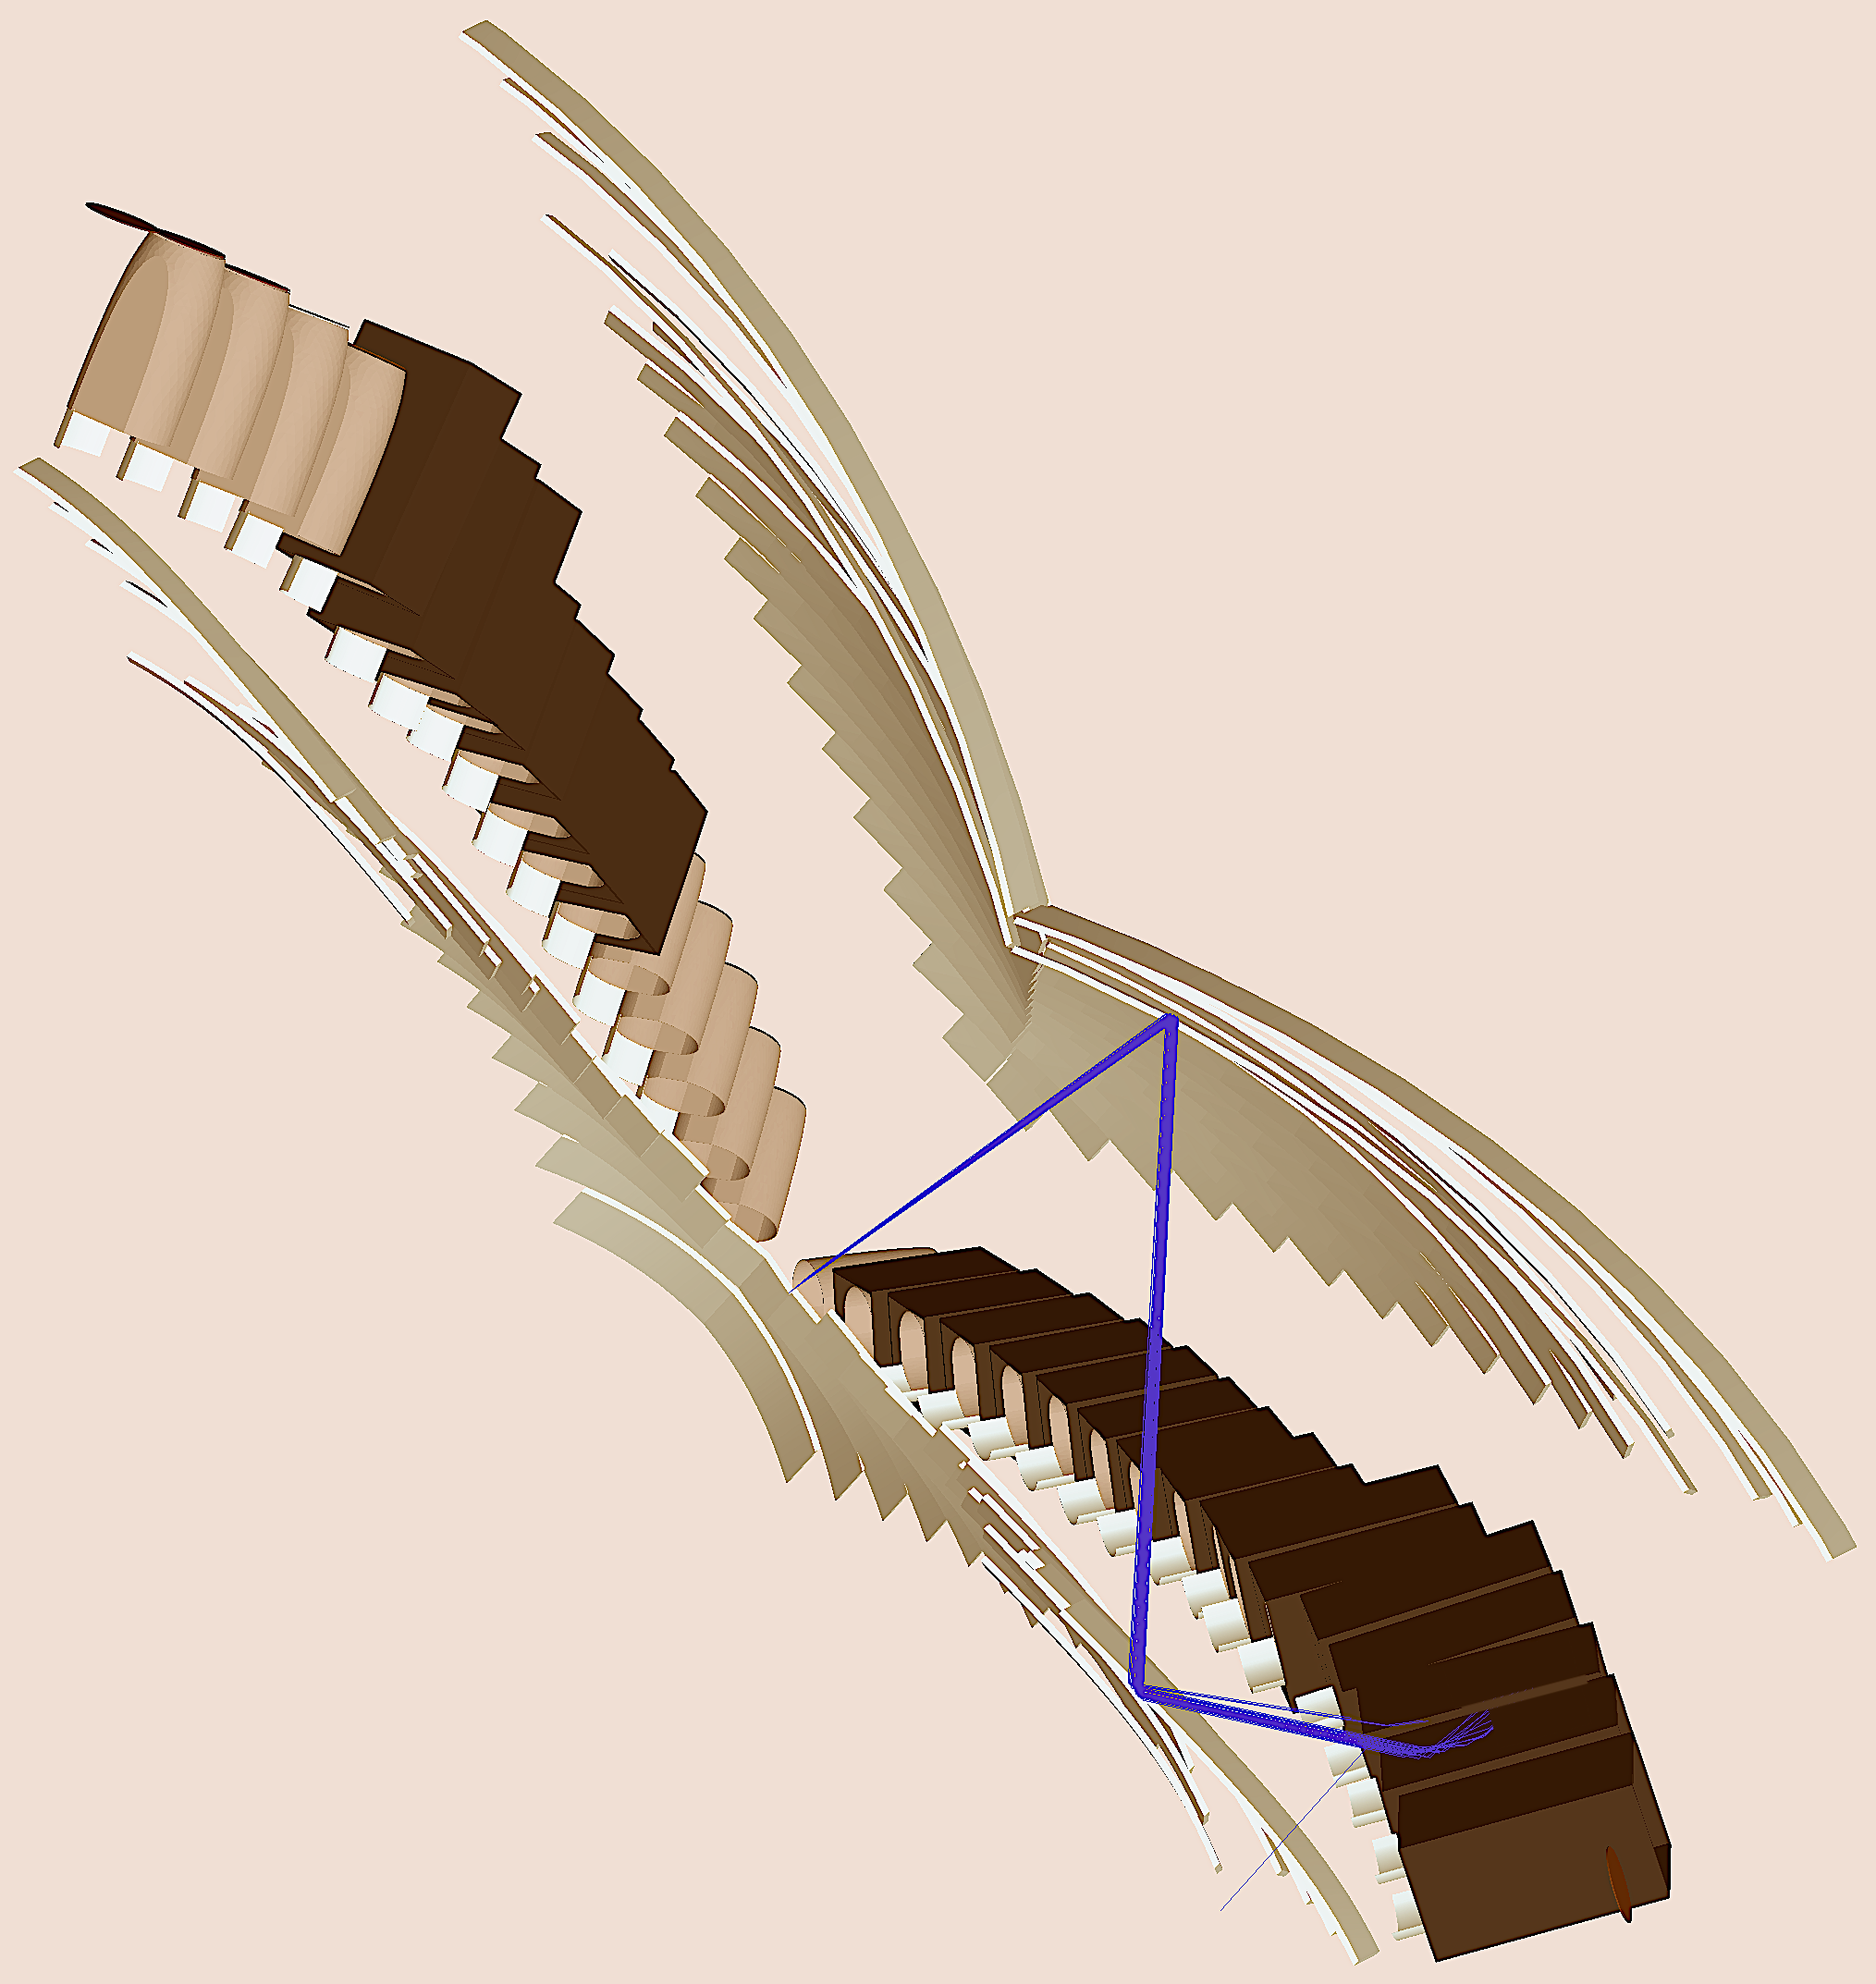
\includegraphics[width=0.99\columnwidth, keepaspectratio]{img/ltccGeometry.png}
	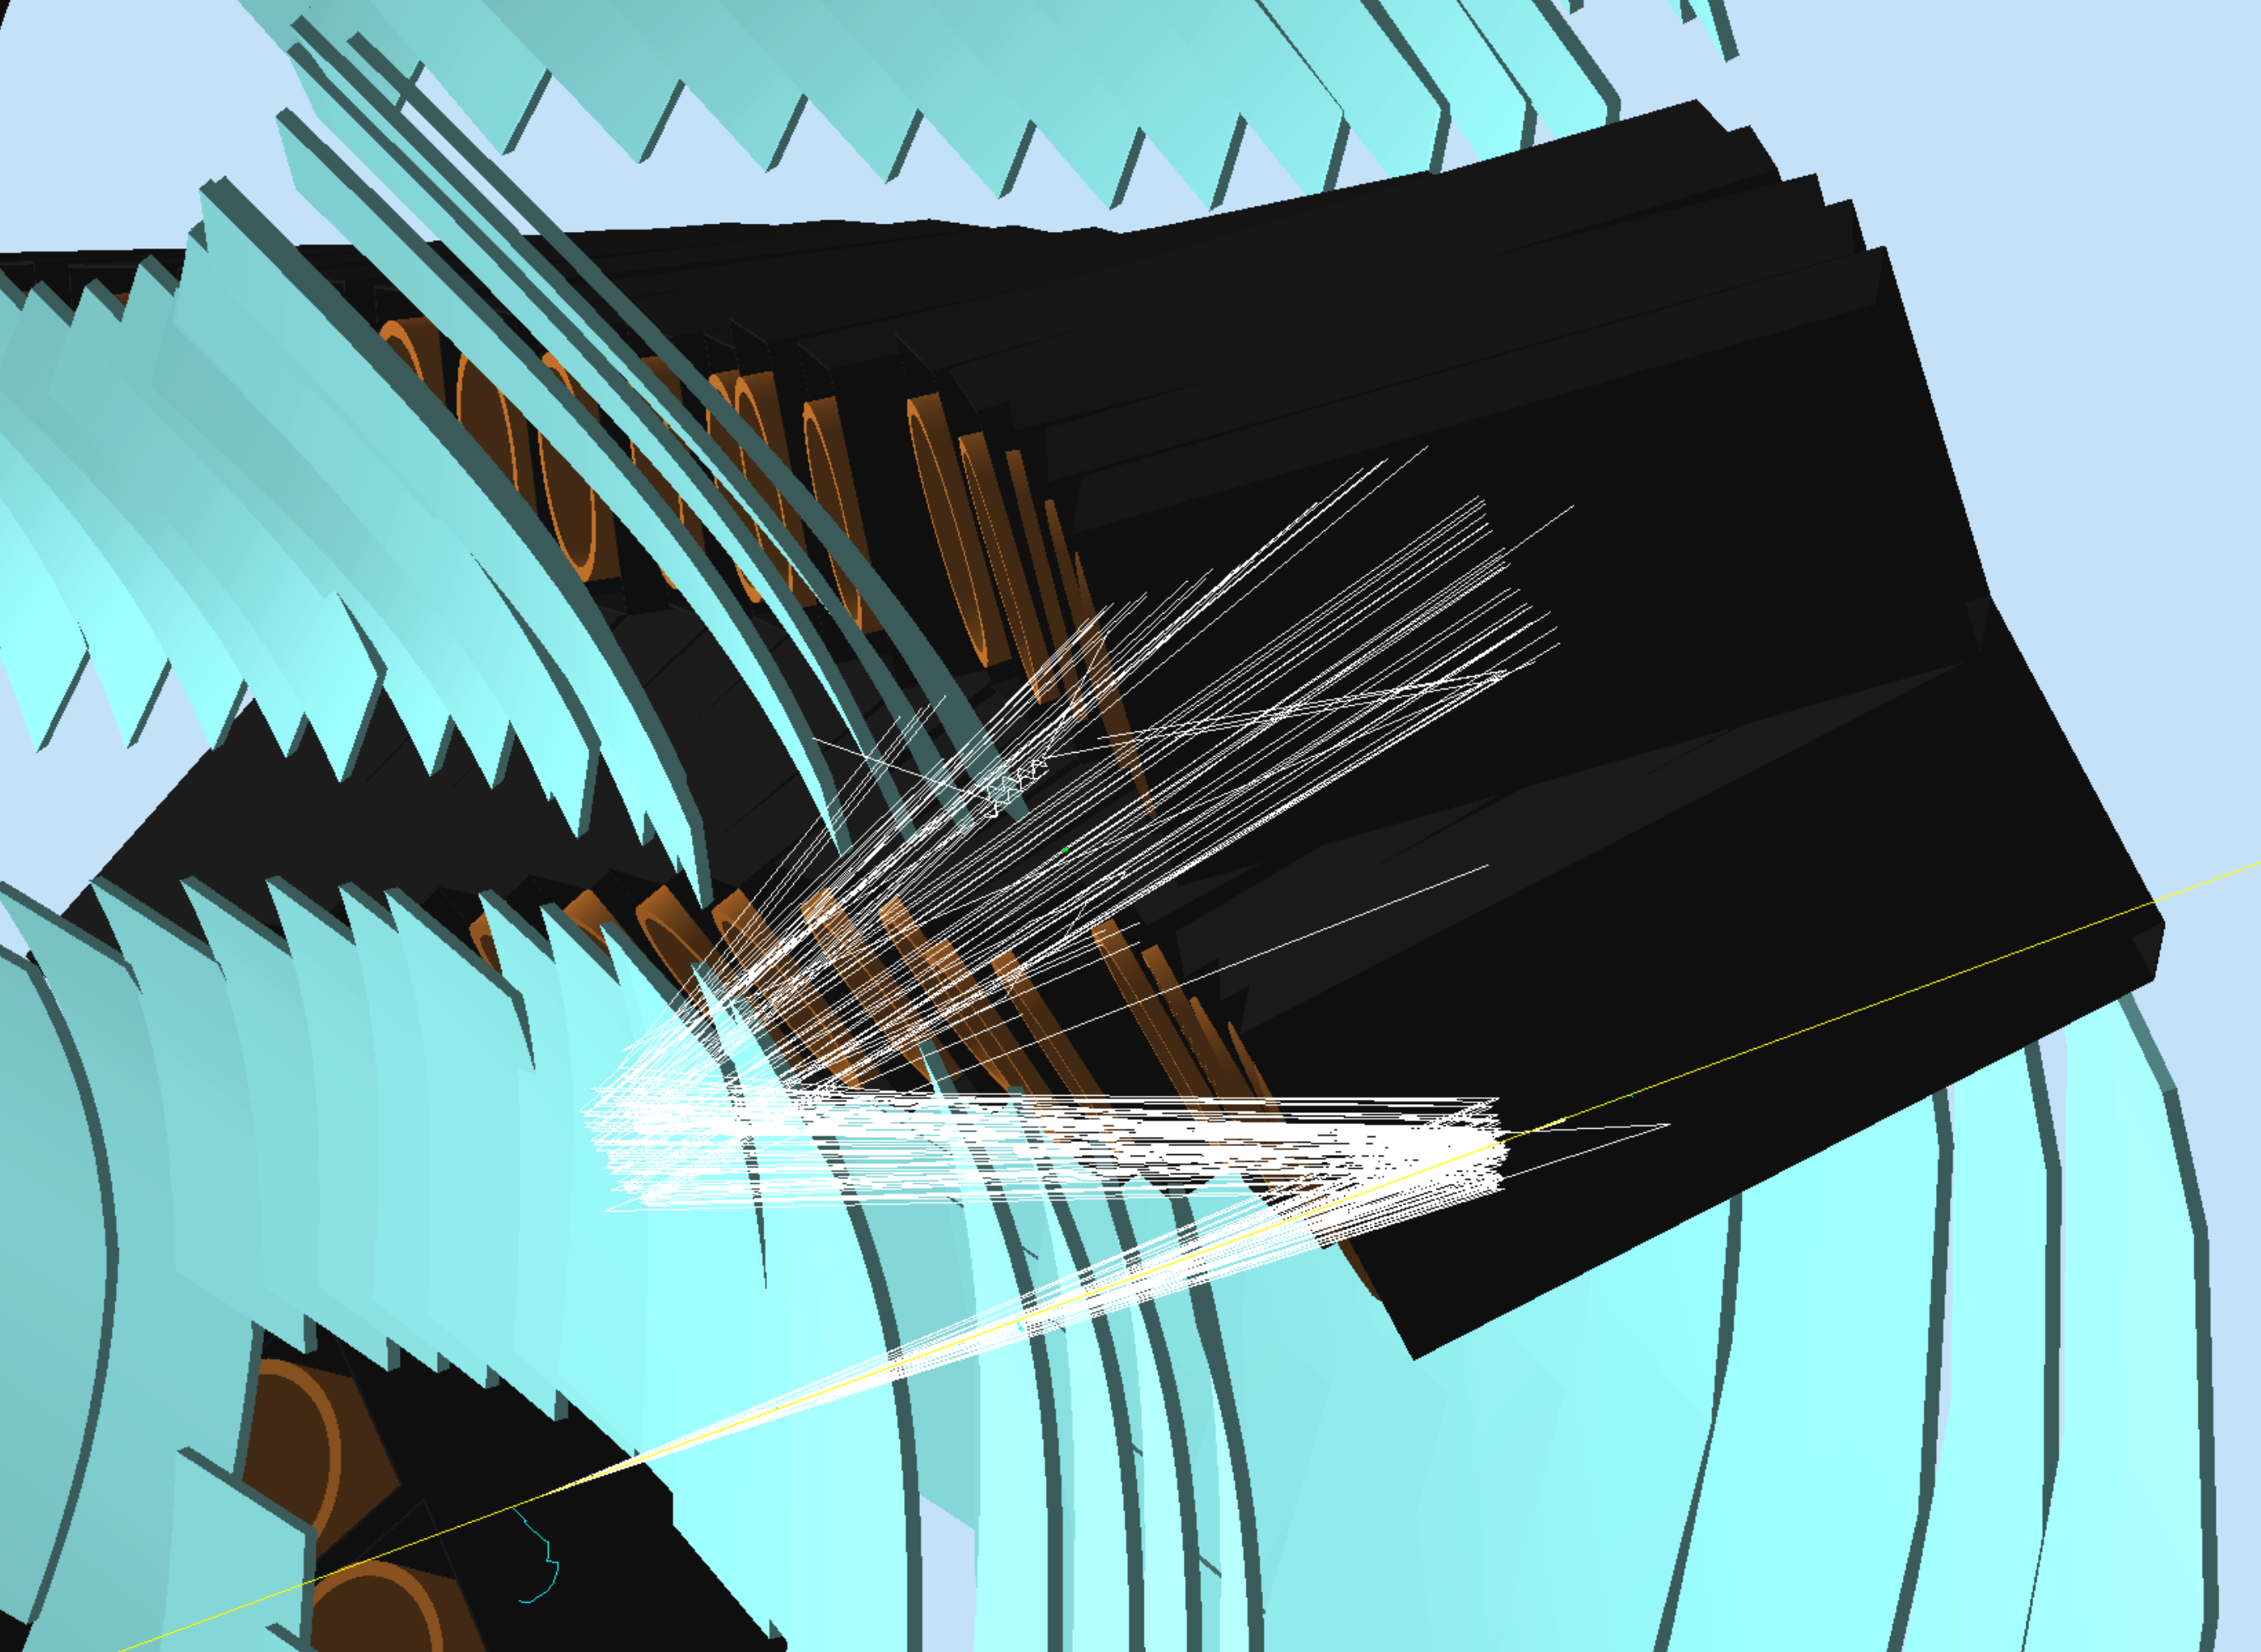
\includegraphics[width=0.99\columnwidth, keepaspectratio]{img/ltccDetail.png}
	\caption{Top: a 6 GeV pion passing through the LTCC gas volume and emitting Cherenkov photons. The light cone
            bounces from the elliptical to the hyperbolic mirrors to the Winston cone, and finally reaches the PMT.
            Bottom: details of the hardware inside the LTCC simulation system: the box frame and the WC are
            imported from CAD. The mirrors, shields, and PMTs are made with Geant4 volumes. One of the PMT shields
            in this picture was removed to show the WC. The PMT is simulated as a disk attached to the WC. }
	\label{fig:ltccGeometry}
\end{figure}

The refractive index of the $C_4F_{10}$ radiator gas and its transparency is included in the material optical properties and taken
into account during the Geant4 transportation of the photons.
Similarly for the reflectivity of the mirrors and Winston cones.
The quantum efficiency associated with the PMT photo-cathodes is taken into account in
the digitization routine.

\subsubsection{Digitization}

Photons that impinge on the PMT faces are processed with the digitization routine.
Each photon collected is input to the quantum efficiency algorithm at its wavelength to decide if it is detected.
The ADC energy is calculated and smeared using the single photo-electron peak position and width from the calibration database.
The time average of all the photons is saved in the output.
The digitized output bank variables are summarized in Table \ref{tab:ltccBank}.

\begin{table}[h]
	\begin{center}
		\begin{tabular}{| c | c | c |}
			\hline \hline
			Variable & Description                                         \\
			\hline
             sector  &                                     CLAS12 sector   \\
               side  &                               left or right index   \\
            segment  &                                           segment   \\
                ADC  &                                               ADC   \\
               time  &                           average time of the hit   \\
               nphe  &                  number of photo-electrons arrived   \\
              npheD  &                 number of photo-electrons detected   \\
               hitn  &                                        hit number   \\
			\hline \hline
		\end{tabular}
	\end{center}
	\caption{The digitized LTCC bank.}\label{tab:ltccBank}
\end{table}

The time window  of the LTCC is set to 5 ns: all Geant4 steps within the same PMT and time window are collected in one hit.
